% algorithms.tex

\section{Proposed RL Algorithms}
\label{sec:algorithms}

This section presents the reinforcement learning controllers evaluated in this work. To establish a baseline, we employ standard implementations of Tabular Q-Learning, Deep Q-Network (DQN), Proximal Policy Optimization (PPO), and Advantage Actor-Critic (A2C) provided by the Stable-Baselines3 (SB3) library~\cite{raffin2021sb3}. These baselines utilize SB3's default \texttt{CombinedExtractor} for parsing the heterogeneous \texttt{Dict} observation space.

In contrast, our proposed Mobility-Channel-Aware PPO (MCA-PPO) replaces the default feature extraction pipeline with a custom dual-branch neural architecture designed specifically for the temporal dynamics of Nakagami-faded FANETs. To benchmark the stability of policy gradients against value-iteration methods in this environment, we also evaluate a similarly augmented Mobility-Channel-Aware Dueling Double DQN (MCA-D3QN). We detail this custom extraction pipeline and the associated training procedures below.

\subsection{Observation Space and MCA Feature Extractor}
\label{sec:mca_extractor}

At each decision step $t$, the controller receives a structured observation:
\begin{equation}
    o(t) = \big[\,\mathbf{x}_s(t),\;\; \mathbf{X}_h(t)\,\big],
    \label{eq:obs}
\end{equation}
where $\mathbf{x}_s(t) \in \mathbb{R}^{14}$ is a scalar state vector encoding current throughput, delay, queue occupancy, SINR, and speed, and $\mathbf{X}_h(t) \in \mathbb{R}^{T \times 14}$ ($T = 5$) is a temporal history window. 

The \emph{Mobility-Channel-Aware} (MCA) feature extractor processes this observation through two parallel branches, as illustrated in Fig.~\ref{fig:comprehensive_pipeline}:
\textbf{Branch~A --- Scalar Encoder (MLP).}
The scalar vector $\mathbf{x}_s$ is processed by a standard two-layer multi-layer perceptron (MLP)~\cite{goodfellow2016deep} utilizing the ReLU activation function and Layer Normalization to yield a 64-dimensional embedding $\mathbf{z}_s$. Layer Normalization stabilizes training under non-stationary observation distributions.

\textbf{Branch~B --- Temporal Encoder (LSTM).}
The history matrix $\mathbf{X}_h = [\mathbf{x}_1, \dots, \mathbf{x}_T]$ is sequentially processed by a standard long short-term memory (LSTM) network~\cite{hochreiter1997long}. The final hidden state $\mathbf{h}_T$ is projected to a 128-dimensional embedding $\mathbf{z}_h$ via a normalized linear layer.

\textbf{Fusion.}
The scalar and temporal embeddings are concatenated and fused:
\begin{equation}
    \mathbf{f} = \sigma\!\big(\text{LN}(W_f [\mathbf{z}_s \,\|\, \mathbf{z}_h] + \mathbf{b}_f)\big) \in \mathbb{R}^{256}.
    \label{eq:fusion}
\end{equation}
This 256-dimensional feature vector $\mathbf{f}$ serves as the shared input to the downstream Q-networks and Actor-Critic heads.

\subsection{MCA-PPO and MCA-D3QN Mechanisms}
\label{sec:mca_mechanisms}

For the proposed \textbf{MCA-PPO} agent (see Fig.~\ref{fig:mcappo}), the feature vector $\mathbf{f}$ feeds an Actor head outputting policy $\pi_\theta(a|s)$ and a Critic head outputting $V_\phi(s)$. The policy is optimized using the clipped surrogate objective to prevent destructively large updates in volatile topological conditions.

\begin{figure*}[t]
    \centering
    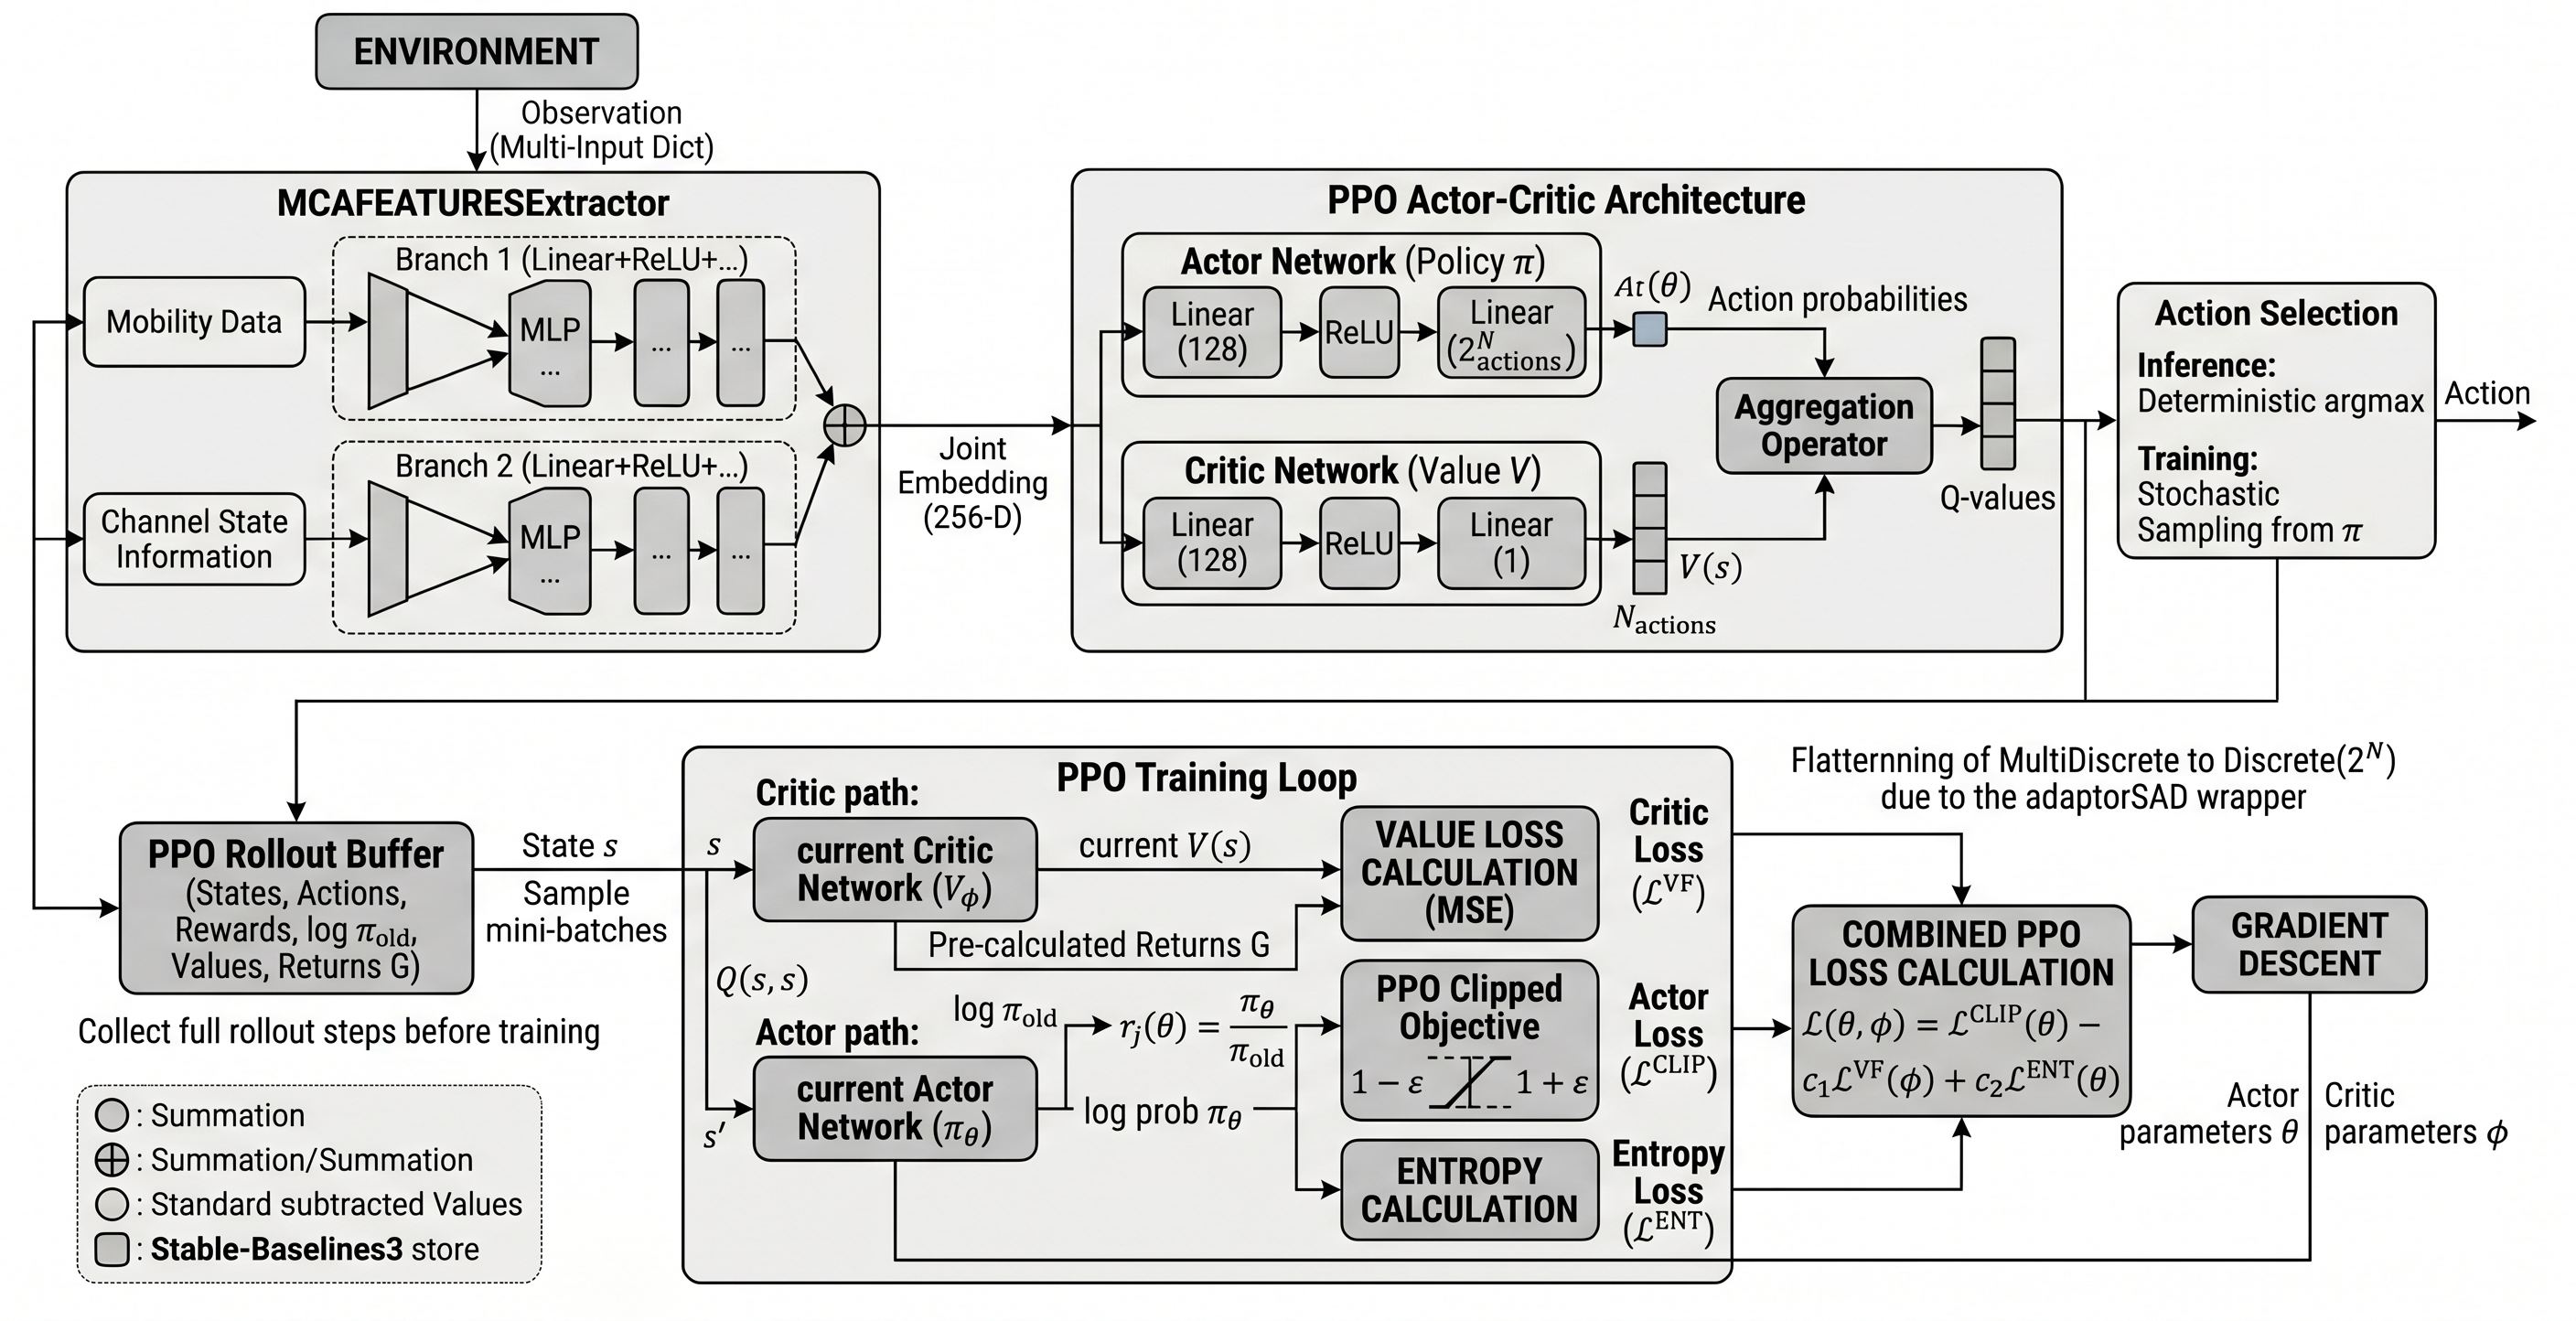
\includegraphics[width=\textwidth, height=6.5cm]{figures/mcappo.png}
    \caption{Architecture of the proposed MCA-PPO model. The fused feature embedding $\mathbf{f}$ is passed to the Actor and Critic heads, optimizing the policy using a clipped surrogate objective to handle FANET topology volatility.}
    \label{fig:mcappo}
\end{figure*}

For the benchmarking \textbf{MCA-D3QN} agent, $\mathbf{f}$ feeds a dueling architecture that decomposes the Q-function into a state-value stream $V(s)$ and an advantage stream $A(s, a)$:
\begin{equation}
    Q(s,a) = V(s) + A(s,a) - \frac{1}{|\mathcal{A}|}\sum_{a' \in \mathcal{A}} A(s,a').
    \label{eq:dueling}
\end{equation}
Training employs Double Q-learning to mitigate overestimation bias by evaluating the greedy action selected by the online network using a slowly updating target network.

The comprehensive training procedure for the MCA agents interacting with the dynamic FANET environment is outlined in Algorithm~\ref{alg:cluster_update}.

\begin{algorithm}[t]
\caption{Decentralized Cluster Update and Burst-Control Execution}
\label{alg:cluster_update}
\begin{algorithmic}[1]
\Require UAV set $\mathcal{U}(t)$, previous clusters $\{\mathcal{C}_k(t-1)\}$, previous leaders $\{\mathcal{L}_k(t-1)\}$, previous graph $\mathcal{G}_{t-1}$, learned Q-functions $\{Q_k\}$
\Ensure Updated clusters $\{\mathcal{C}_k(t)\}$, leaders $\{\mathcal{L}_k(t)\}$, graph $\mathcal{G}_t$, actions $\{\hat{a}_k(t)\}$, rewards $\{r_k(t)\}$
\State \textbf{Cluster update.}
\For{each UAV $i \in \mathcal{U}(t)$}
    \State Update assignment $\chi_i(t)$ using hysteresis threshold \eqref{eq:hysteresis}.
\EndFor
\State Form clusters $\{\mathcal{C}_k(t)\}$ from assignments $\{\chi_i(t)\}$.
\For{each active cluster $\mathcal{C}_k(t)$}
    \If{$|\mathcal{C}_k(t)| > N_{\text{split}}^{\max}$}
        \State Split $\mathcal{C}_k(t)$.
    \EndIf
    \If{$|\mathcal{C}_k(t)| < N_{\text{merge}}^{\min}$}
        \State Merge $\mathcal{C}_k(t)$ with a compatible cluster.
    \EndIf
    \If{$\Omega_k^{\text{fail}}(t) = 1$}
        \State Update $\mathcal{L}_k(t)$ using cluster-head health score \eqref{eq:ch_score}.
    \EndIf
\EndFor
\State Construct $\mathcal{G}_t = (\mathcal{V}_t, \mathcal{E}_t)$ by establishing inter-cluster links.
\State \textbf{Decentralized burst-control execution.}
\For{each cluster-head $k \in \mathcal{V}_t$}
    \State Form local observation $o_k(t)$.
    \State $\hat{u}_k(t) \leftarrow \arg\max_{u \in \mathcal{A}_k} Q_k(o_k(t), u)$.
    \State $\hat{a}_k(t) = (m_k(t), \rho_k(t)) \leftarrow \text{dec}(\hat{u}_k(t))$.
    \State $T_{1,k} \leftarrow \rho_k(t) t_{\text{burst}}$, $T_{2,k} \leftarrow (1 - \rho_k(t)) t_{\text{burst}}$.
\EndFor
\State Execute intra-cluster service over $\{T_{1,k}\}_{k \in \mathcal{V}_t}$.
\State Execute inter-cluster coordination over $\{T_{2,k}\}_{k \in \mathcal{V}_t}$ on $\mathcal{G}_t$.
\State Update queues, coordination backlogs, and rewards $\{r_k(t)\}_{k \in \mathcal{V}_t}$.
\State \Return $\{\mathcal{C}_k(t)\}$, $\{\mathcal{L}_k(t)\}$, $\mathcal{G}_t$, $\{\hat{a}_k(t)\}$, $\{r_k(t)\}$.
\end{algorithmic}
\end{algorithm}
